\documentclass[12pt,a4paper]{report}
\usepackage[latin1]{inputenc}
\usepackage{amsmath}
\usepackage{amsfonts}
\usepackage{subfigure}
\usepackage{amssymb}
\usepackage[pdftex]{graphicx}
\begin{document}
 
\def\scale{4}
\noindent 
Data: YouTube clips, down-sampled to 3x32x32 and sub-sampled in time to 12fps (~0.5 seconds between frames). \\
Experiment: $L_2$ pooling in groups of four across features only (no spatial pooling). Constant individual $L_1$ penalty in all experiments while increasing the slowness penalty. 
Clearly, slowness does have an effect in the organization of the groups.    
\begin{figure}[h]
\centering
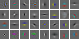
\includegraphics[scale=\scale]{SF01.png}
\caption{\emph{Slowness weight = 0.1}}
\end{figure} 

\begin{figure}[h]
\centering
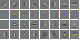
\includegraphics[scale=\scale]{SF02.png}
\caption{\emph{Slowness weight = 0.2}}
\end{figure} 

\begin{figure}[h]
\centering
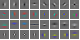
\includegraphics[scale=\scale]{SF05.png}
\caption{\emph{Slowness weight = 0.5}}
\end{figure} 

\begin{figure}[h]
\centering
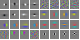
\includegraphics[scale=\scale]{SF10.png}
\caption{ \emph{Slowness weight = 1}}
\end{figure} 

\begin{figure}[h]
\centering
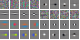
\includegraphics[scale=\scale]{SF20.png}
\caption{ \emph{Slowness weight = 2}}
\end{figure} 

\begin{figure}[h]
\centering
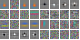
\includegraphics[scale=\scale]{SF40.png}
\caption{ \emph{Slowness weight = 4}}
\end{figure} 

\begin{figure}[h]
\centering
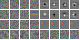
\includegraphics[scale=\scale]{SF50.png}
\caption{ \emph{Slowness weight = 5}}
\end{figure} 

\begin{figure}[h]
\centering
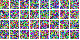
\includegraphics[scale=\scale]{SF100.png}
\caption{ \emph{Slowness weight = 10}}
\end{figure} 


\end{document} 